%%%%%%%%%%%%%%%%%%%%%%%%%%%%%%%%%%%%%%%%%%%%%%%
%%%     Declarations (skip to Begin Document, line 112, for parts you fill in)
%%%%%%%%%%%%%%%%%%%%%%%%%%%%%%%%%%%%%%%%%%%%%%%

\documentclass[10pt]{article}

\usepackage{geometry}  % Lots of layout options.  See http://en.wikibooks.org/wiki/LaTeX/Page_Layout
\geometry{letterpaper}  % ... or a4paper or a5paper or ... 
\usepackage{fullpage}  % somewhat standardized smaller margins (around an inch)
\usepackage{setspace}  % control line spacing in latex documents
\usepackage[parfill]{parskip}  % Activate to begin paragraphs with an empty line rather than an indent

\usepackage{amsmath,amssymb}  % latex math
\usepackage{empheq} % http://www.ctan.org/pkg/empheq
\usepackage{bm,upgreek}  % allows you to write bold greek letters (upper & lower case)

\usepackage{url}

% for typsetting algorithm pseudocode see http://en.wikibooks.org/wiki/LaTeX/Algorithms_and_Pseudocode
\usepackage{algorithmic,algorithm}  

\usepackage{graphicx}  % inclusion of graphics; see: http://en.wikibooks.org/wiki/LaTeX/Importing_Graphics
% allow easy inclusion of .tif, .png graphics
\DeclareGraphicsRule{.tif}{png}{.png}{`convert #1 `dirname #1`/`basename #1 .tif`.png}

\usepackage{xspace}
\newcommand{\latex}{\LaTeX\xspace}

\usepackage{color}  % http://en.wikibooks.org/wiki/LaTeX/Colors

\long\def\ans#1{{\color{blue}{\em #1}}}
\long\def\ansnem#1{{\color{blue}#1}}
\long\def\boldred#1{{\color{red}{\bf #1}}}

% Useful package for syntax highlighting of specific code (such as python) -- see below
\usepackage{listings}  % http://en.wikibooks.org/wiki/LaTeX/Packages/Listings
\usepackage{textcomp}

%%% The following lines set up using the listings package
\renewcommand{\lstlistlistingname}{Code Listings}
\renewcommand{\lstlistingname}{Code Listing}

%%% Specific for python listings
\definecolor{gray}{gray}{0.5}
\definecolor{green}{rgb}{0,0.5,0}

\lstnewenvironment{python}[1][]{
\lstset{
language=python,
basicstyle=\footnotesize,  % could also use this -- a little larger \ttfamily\small\setstretch{1},
stringstyle=\color{red},
showstringspaces=false,
alsoletter={1234567890},
otherkeywords={\ , \}, \{},
keywordstyle=\color{blue},
emph={access,and,break,class,continue,def,del,elif ,else,%
except,exec,finally,for,from,global,if,import,in,i s,%
lambda,not,or,pass,print,raise,return,try,while},
emphstyle=\color{black}\bfseries,
emph={[2]True, False, None, self},
emphstyle=[2]\color{green},
emph={[3]from, import, as},
emphstyle=[3]\color{blue},
upquote=true,
morecomment=[s]{"""}{"""},
commentstyle=\color{gray}\slshape,
emph={[4]1, 2, 3, 4, 5, 6, 7, 8, 9, 0},
emphstyle=[4]\color{blue},
literate=*{:}{{\textcolor{blue}:}}{1}%
{=}{{\textcolor{blue}=}}{1}%
{-}{{\textcolor{blue}-}}{1}%
{+}{{\textcolor{blue}+}}{1}%
{*}{{\textcolor{blue}*}}{1}%
{!}{{\textcolor{blue}!}}{1}%
{(}{{\textcolor{blue}(}}{1}%
{)}{{\textcolor{blue})}}{1}%
{[}{{\textcolor{blue}[}}{1}%
{]}{{\textcolor{blue}]}}{1}%
{<}{{\textcolor{blue}<}}{1}%
{>}{{\textcolor{blue}>}}{1},%
%framexleftmargin=1mm, framextopmargin=1mm, frame=shadowbox, rulesepcolor=\color{blue},#1
framexleftmargin=1mm, framextopmargin=1mm, frame=single,#1
}}{}
%%% End python code listing definitions

%%% Specific for matlab listings
\definecolor{dkgreen}{rgb}{0,0.6,0}
\definecolor{gray}{rgb}{0.5,0.5,0.5}
\definecolor{mauve}{rgb}{0.58,0,0.82}
 
\lstnewenvironment{matlab}[1][]{
\lstset{ %
  language=Matlab,                % the language of the code
  basicstyle=\footnotesize,           % the size of the fonts that are used for the code
  numbers=left,                   % where to put the line-numbers
  numberstyle=\tiny\color{gray},  % the style that is used for the line-numbers
  stepnumber=2,                   % the step between two line-numbers. If it's 1, each line 
                                  % will be numbered
  numbersep=5pt,                  % how far the line-numbers are from the code
  backgroundcolor=\color{white},      % choose the background color. You must add \usepackage{color}
  showspaces=false,               % show spaces adding particular underscores
  showstringspaces=false,         % underline spaces within strings
  showtabs=false,                 % show tabs within strings adding particular underscores
  frame=single,                   % adds a frame around the code
  rulecolor=\color{black},        % if not set, the frame-color may be changed on line-breaks within not-black text (e.g. commens (green here))
  tabsize=2,                      % sets default tabsize to 2 spaces
  captionpos=t,                   % sets the caption-position to top
  breaklines=true,                % sets automatic line breaking
  breakatwhitespace=false,        % sets if automatic breaks should only happen at whitespace
  title=\lstname,                   % show the filename of files included with \lstinputlisting;
                                  % also try caption instead of title
  keywordstyle=\color{blue},          % keyword style
  commentstyle=\color{dkgreen},       % comment style
  stringstyle=\color{mauve},         % string literal style
  escapeinside={\%*}{*)},            % if you want to add LaTeX within your code
  morekeywords={*,...}               % if you want to add more keywords to the set
  framexleftmargin=1mm, framextopmargin=1mm, frame=single,#1 % display caption
} }{}
%%% End matlab code listing definitions

%% hilite
\newcommand{\hilite}[1]{\colorbox{yellow}{#1}}
\long\def\todo#1{\hilite{{\bf TODO:} {\em #1}}}


%%%%%%%%%%%%%%%%%%%%%%%%%%%%%%%%%%%%%%%%%%%%%%%
%%%     Begin Document
%%%%%%%%%%%%%%%%%%%%%%%%%%%%%%%%%%%%%%%%%%%%%%%

\begin{document}

\begin{center}
    {\Large {\bf ISTA 421 / INFO 521 -- Homework 2}} \\
    \boldred{Due: Friday, Sept 14, 5pm} \\
    15 points total Undergraduate / 20 points total Graduate

\end{center}

\begin{flushright}
Ken Youens-Clark 

Graduate
\end{flushright}


%%%%%%%%%%%%%%%%
%%%     Problems
%%%%%%%%%%%%%%%%

\begin{itemize}



%%%     Problem 1
\item[1.] [3 points]
Adapted from {\bf Exercise 1.2} of FCMA p.35:

Write a Python script that can find the parameters $\mathbf{w}$ (a vector of parameters) for an arbitrary dataset of $x_n, t_n$ pairs.  You will use this script to complete Exercise 2, which only requires fitting a simple line to the data (i.e., you only need to fit parameters $w_0$ and $w_1$); however, in problem 5 you will need to fit higher-order polynomial models (e.g., $t = w_0 + w_1x + w_2x^2 + ...$), so you must make your script here generalized to handle higher-order polynomials.  The script {\tt fitpoly\_incomplete.py} is provided to help get you started.  {\tt fitpoly\_incomplete.py} provides helper functions to read data, plot data, and plot the model (once you've determined the weight vector $\mathbf{w}$), but the function for computing linear least-squares fit, {\tt fitpoly} (starting on line 166), is {\em incomplete}.  {\tt fitpoly} takes as input the (one-dimensional) data vector $\mathbf{x}$, the target values vector $\mathbf{t}$, and a non-negative integer {\tt model\_order}, which represents the highest polynomial order term of the model; {\tt fitpoly} is intended to return the $\mathbf{w}$ vector (as a numpy array).

Recommended: (If needed) review the Appendix to HW 1, the brief tutorial to numpy arrays!

{\bf Just to state the obvious}: the objective of this exercise is for you to implement the linear least squares fit solution (i.e., the normal equation) in their general linear algebra form.  {\bf DO NOT} use existing least squares solvers, such as {\tt numpy.linalg.lstsq}, or scikit learn's \\{\tt sklearn.linear\_model.LogisticRegression} as your implemented solution; however, it is certainly fine to use these to help {\em verify} your implementation's output.

You will submit your script as a stand-alone file called {\tt fitpoly.py}.

\begin{verbatim}
$ ./fitpoly.py -h
usage: fitpoly.py [-h] [-m int] [-t str] [-x str] [-y str] [-o str] [-s] [-q]
                  FILE

Find w-hat

positional arguments:
  FILE                  csv data file

optional arguments:
  -h, --help            show this help message and exit
  -m int, --model_order int
                        Model order (default: 1)
  -t str, --title str   Plot title (default: Data)
  -x str, --xlabel str  X axis label (default: x)
  -y str, --ylabel str  Y axis label (default: t)
  -o str, --outfile str
                        Save output to filename (default: None)
  -s, --scale           Whether to scale the data (default: False)
  -q, --quiet           Do not show debug messages (default: False)
\end{verbatim}

%%%     Problem 2
\item[2.] [2 point]
Adapted from {\bf Exercise 1.6} of FCMA p.35:

Table 1.3 (p.13) of FCMA lists the women's 100m gold medal Olympic results -- this data is provided in the file {\tt womens100.csv} in the data folder.  Using your script from problem 1, find the 1st-order polynomial model (i.e., a line with parameters $w_0$ and $w_1$) that minimizes the squared loss of this data.  Report the model here as an equation.  Plot the data with your best-first model and include the plot in your answer (label axes and include an informative caption!).

{\bf Solution.} 

The weights for the best fit are:

\begin{eqnarray*}
\mathbf{w}^\top = \begin{bmatrix} 40.924155 & -0.015072 \end{bmatrix}
\end{eqnarray*}

\begin{figure}[H]
\centering
  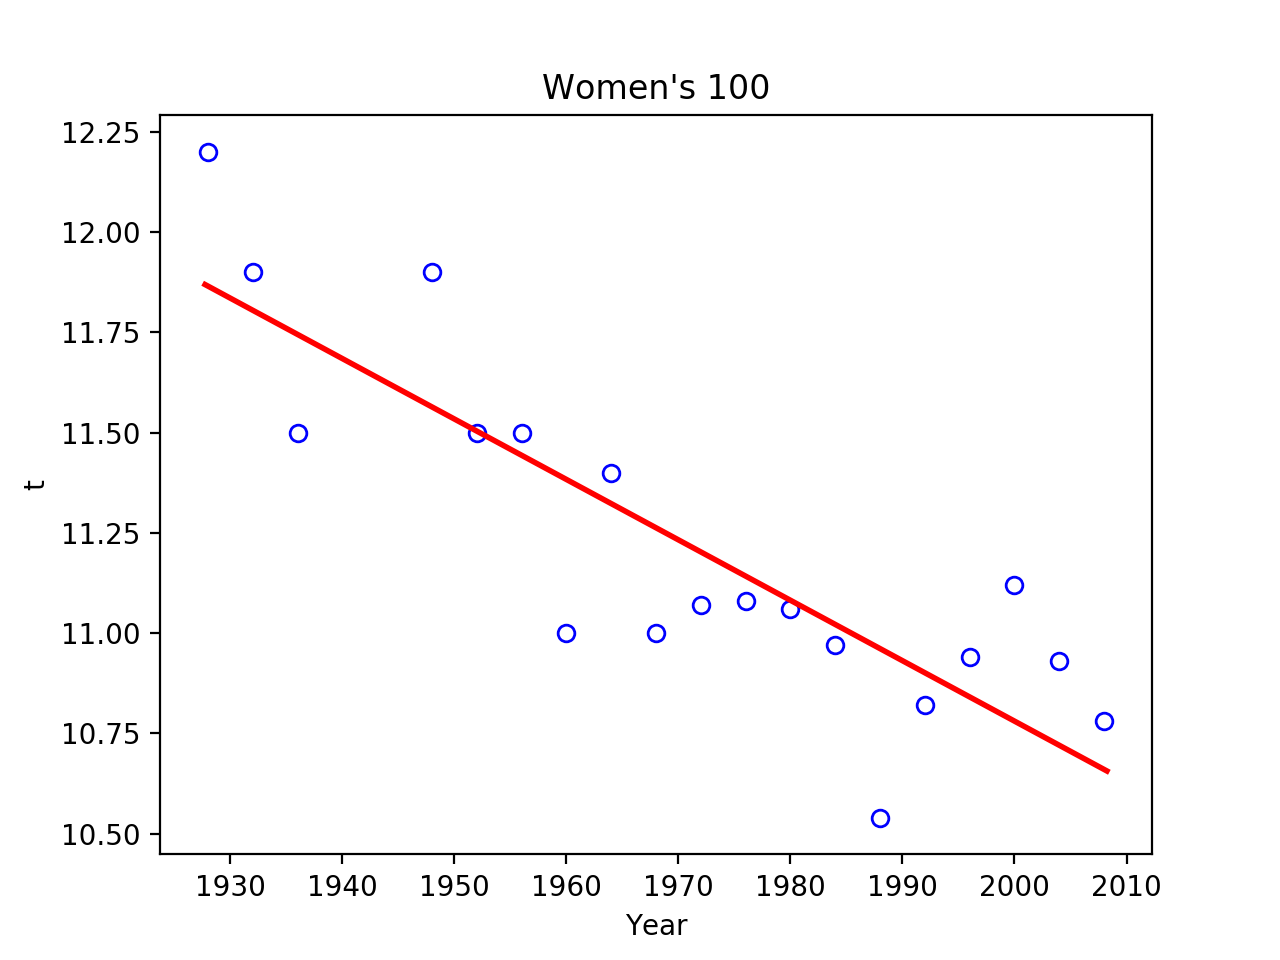
\includegraphics[width=\linewidth]{code/womens.png}
 \caption{Women's best fit (1st order)}
\label{label}
\end{figure}


%%%     Problem 3
\item[3.] [2 point]
Adapted from {\bf Exercise 1.9} of FCMA p.36:

Use your python script from problem 1 to load the data stored in the file {\tt synthdata2018.csv} (in the data folder).  Fit a 3rd order polynomial function -- $f(x; \mathbf{w}) = w_0 + w_1 x + w_2 x^2 + w_3 x^3$ -- to this data (if you extended the {fitpoly\_incomplete.py} script, then {\tt model\_order}$ = 3$).  
Report the best-fit model parameters as an equation.  Plot the data and your model and include the plot in your answer (be sure to include an informative caption to your plot).

{\bf Solution.} 

The weights for the best fit are:

\begin{eqnarray*}
\mathbf{w}^\top = \begin{bmatrix} -12.77102013 & 10.19891444 & 5.13913951 & 0.50819653 \end{bmatrix}
\end{eqnarray*}

\begin{figure}[H]
\centering
  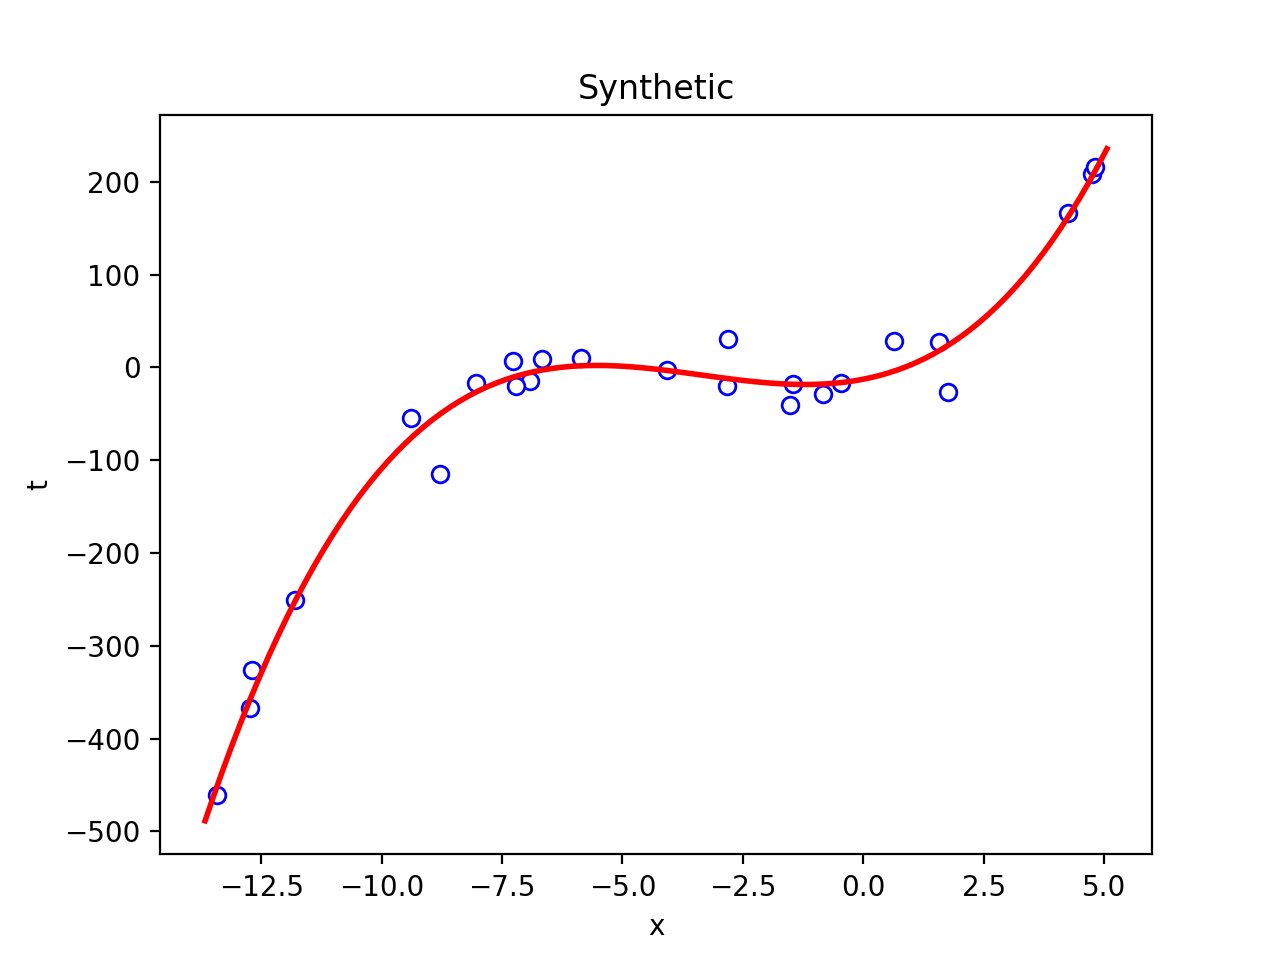
\includegraphics[width=\linewidth]{code/synth.png}
 \caption{Synthetic best fit (3rd order polynomial)}
\label{label}
\end{figure}

%%%     Problem 4
\item[4.] [8 points]
Write a script that implements K-fold cross-validation to choose the polynomial order (between orders 0 and 7) with the best predictive error for the {\tt synthdata2018.csv}.  The provided script {\tt cv\_demo\_incomplete.py} implements the synthetic data experiment described in Ch 1 (pp.31-32) of the book; you are welcome to use and adapt any part of this code you like; keep in mind that this script won't successfully execute until you add the general (matrix form) normal equation calculation on line 339.
Note also that in the synthetic data experiment in {\tt cv\_demo\_incomplete.py}, 1000 test data points are generated in addition to the 100 data points used for 10-fold cross-validation in the demo; for this problem (problem 4), you won't have this independent test set, only the data from {\tt synthdata2018.csv} on which to perform K-fold cross-validation.  Also, for this problem, you will perform 5-fold cross-validation, in addition to Leave-One-Out-CV (LOOCV).

Run your script with 5-fold cross-validation and LOOCV multiple times, each while randomizing the order of the data (see the {\tt randomize\_data} option of the {\tt run\_cv} function).
Which model order do the two cross-validation methods predict as the best order for predictive accuracy?
Do the two different cross-validation runs always agree?

Report the best-fit model parameters for the best model order according to LOOCV, and plot this model with the data.
Include a plot of the training loss and CV-loss for the 8 different (0..7) polynomial model orders for {\bf one example each} of 5-fold cross-validation and LOOCV (i.e., you will include four plots: (1) 5-fold CV and (2) related training loss, (3) LOOCV, and (4) related training loss).  You can use the provided {\tt plot\_cv\_results} to plot the training loss and CV loss (whether 5-fold or LOOCV) as a pair of plots.

You will submit your script as a stand-alone file called {\tt cv.py}

{\bf Solution.} 

Both models report order 3 as the best fit. In my runs, they have almost always agreed on this order but sometimes CV would report 4.

\begin{figure}[H]
\centering
  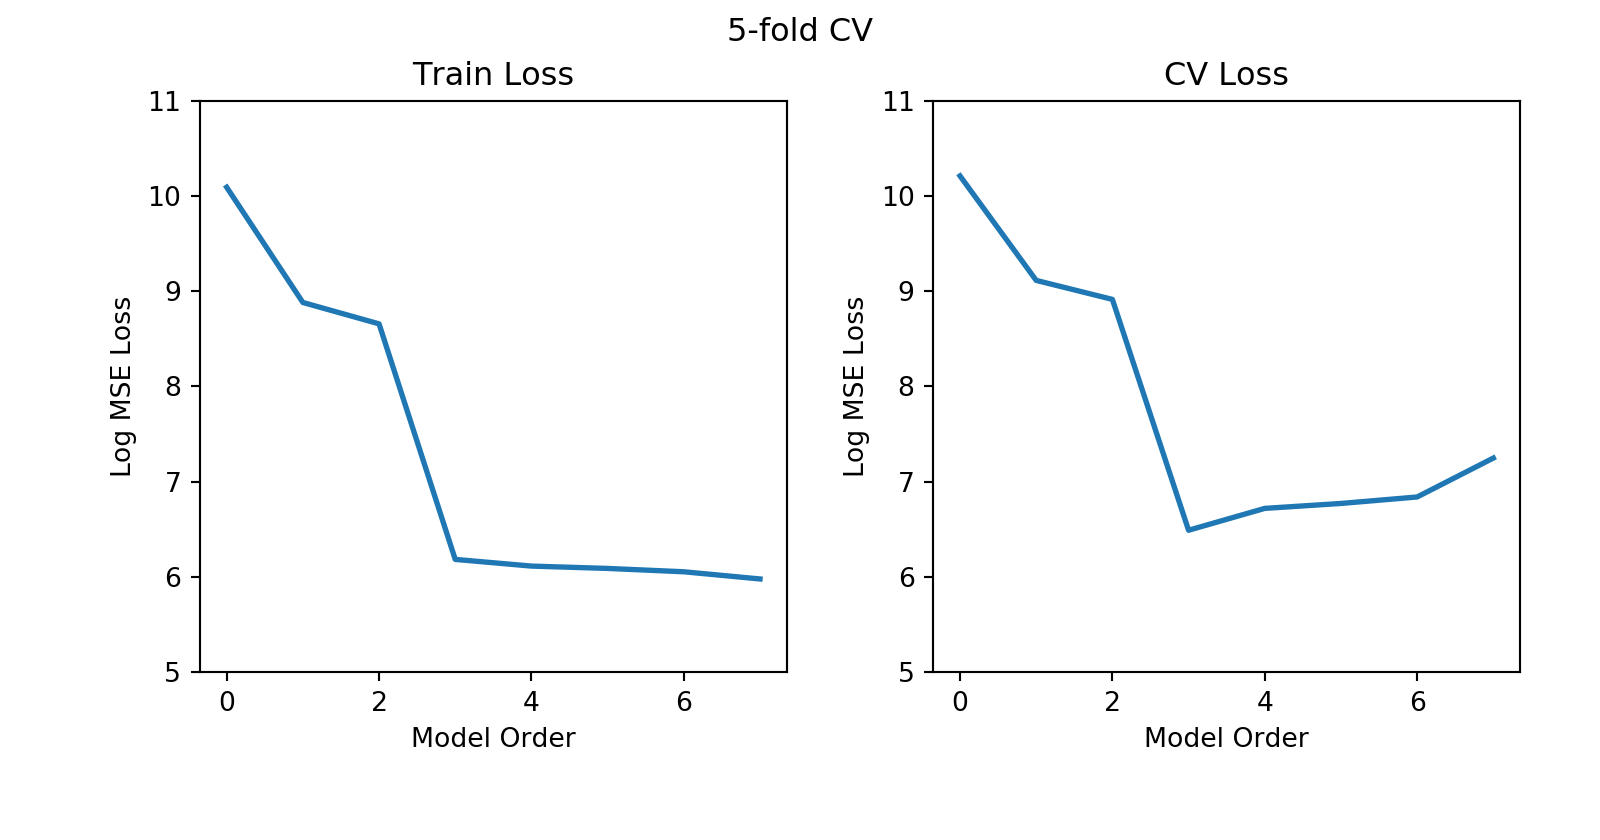
\includegraphics[width=\linewidth]{code/loss_5cv_o7_r1.png}
 \caption{5-fold cross validation}
\label{label}
\end{figure}

\begin{figure}[H]
\centering
  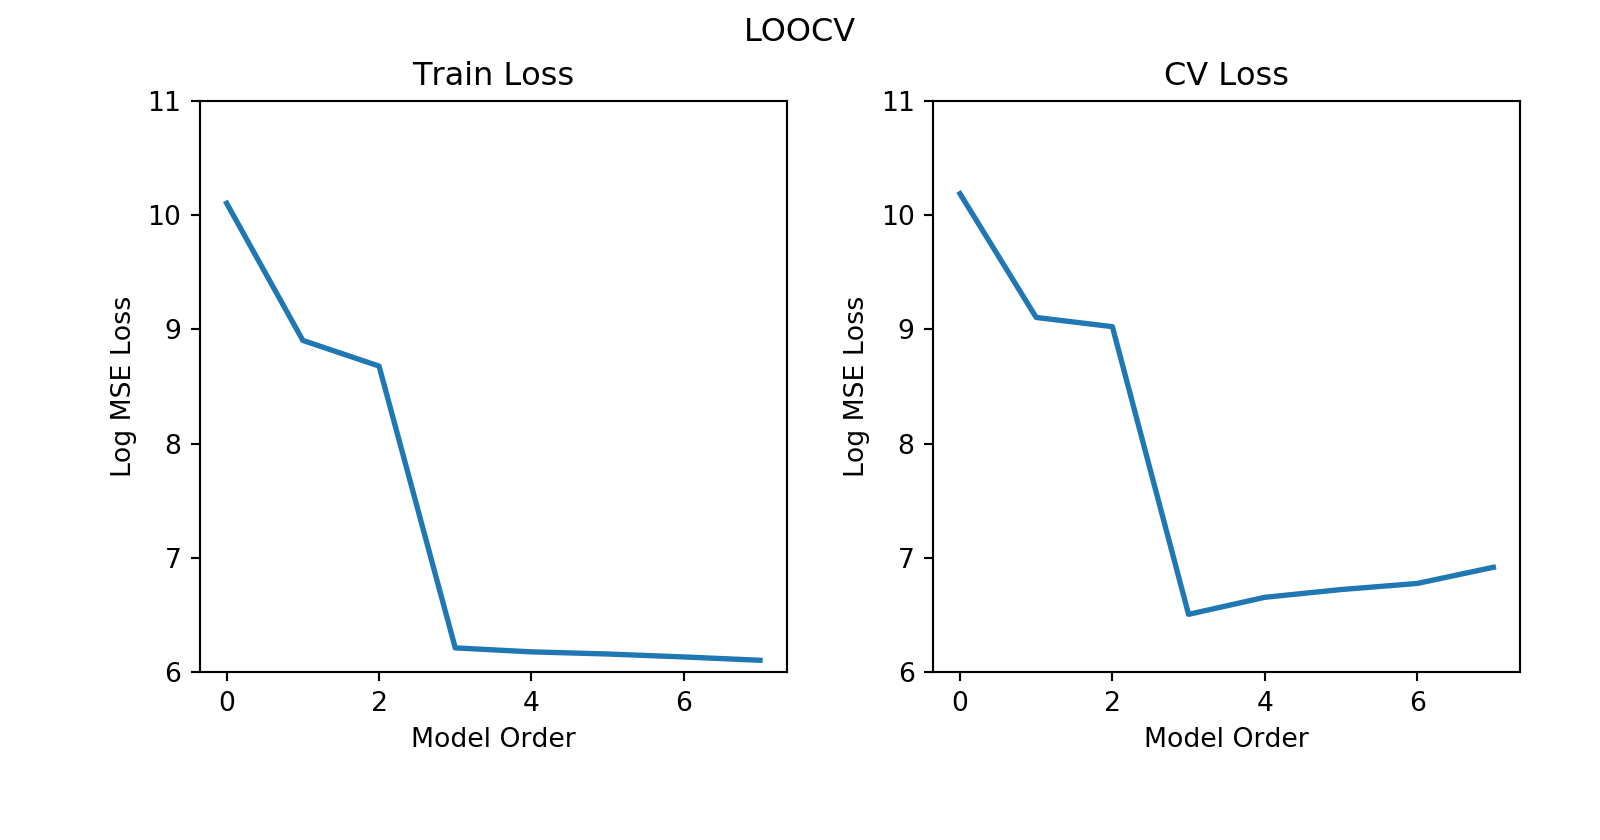
\includegraphics[width=\linewidth]{code/loss_loocv_o7_r1.png}
 \caption{Leave-one-out cross validation}
\label{label}
\end{figure}

\begin{figure}[H]
\centering
  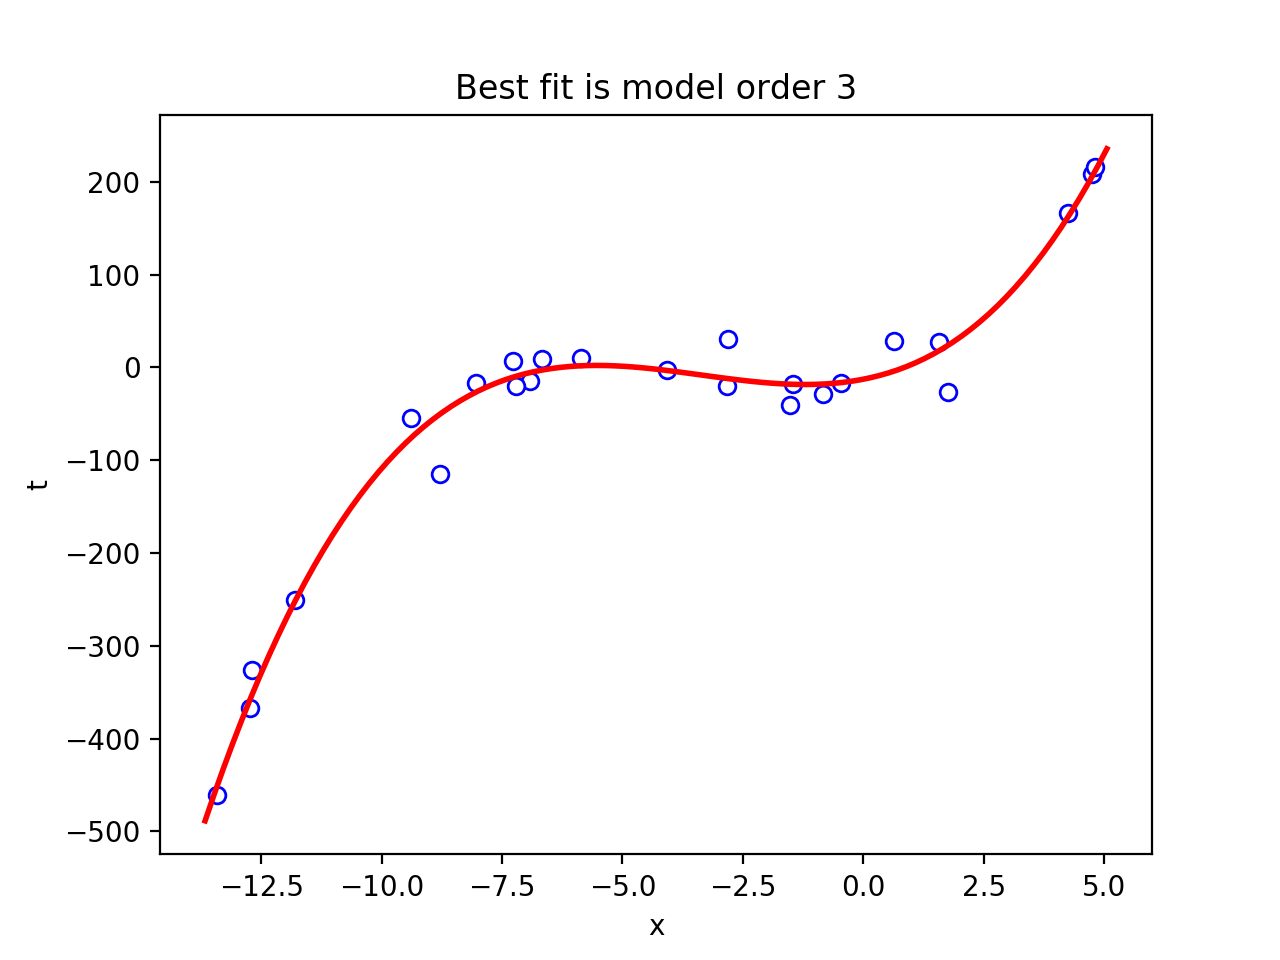
\includegraphics[width=\linewidth]{code/cv-best-fit.png}
 \caption{Plot of all data using best order (3rd)}
\label{label}
\end{figure}

%%%     Problem 5
\item[5.] [2 points -- {\bf Required only for Graduates}] 
{\bf Exercise 1.10} from FCMA p.36

Derive the optimal least squares parameter value, $\mathbf{\hat{w}}$, for the total training loss:
\begin{eqnarray*}
\mathcal{L} = \sum_{n=1}^N \left( t_n - \mathbf{w}^\top \mathbf{x}_n \right)^2
\end{eqnarray*}

How does the expression compare with that derived from the average (mean) loss?  (Hint: Express this loss in the {\bf full} matrix form and derive the normal equation.)

{\bf Solution.} 

\begin{eqnarray*}
\begin{aligned}
\mathcal{L} &= \sum_{n=1}^N \left( t_n - \mathbf{w}^\top \mathbf{x}_n \right)^2
\\
&= (\mathbf{t} - \mathbf{X} \mathbf{w})^\top (\mathbf{t} - \mathbf{X} \mathbf{w})
\\
&= (\mathbf{X} \mathbf{w} - \mathbf{t})^\top (\mathbf{X} \mathbf{w} - \mathbf{t})
\\
&= ((\mathbf{X} \mathbf{w})^\top - \mathbf{t}^\top) (\mathbf{X} \mathbf{w} - \mathbf{t})
\\
&= ((\mathbf{X} \mathbf{w})^\top \mathbf{X} \mathbf{w} 
 - \mathbf{t}^\top \mathbf{X} \mathbf{w} 
 - (\mathbf{X} \mathbf{w})^\top \mathbf{t}
 + \mathbf{t}^\top \mathbf{t}
\\
&= \mathbf{w}^\top \mathbf{X}^\top \mathbf{X} \mathbf{w} 
 - 2 \mathbf{w}^\top \mathbf{X}^\top \mathbf{t} 
 + \mathbf{t}^\top \mathbf{t}
\\
\frac { \partial \mathcal{L}} {\partial \mathbf{w}} &=
 2 \mathbf{X}^\top \mathbf{X} \mathbf{w} - 2 \mathbf{X}^\top \mathbf{t} = 0
\\
\mathbf{X}^\top \mathbf{X} \mathbf{w} &= \mathbf{X}^\top \mathbf{t}
\\
\mathbf{I} \mathbf{w} &= (\mathbf{X}^\top \mathbf{X})^{-1} \mathbf{X}^\top \mathbf{t}
\end{aligned}
\end{eqnarray*}

The answer is the same as for the mean, so averaging has no effect on the outcome.

%%%     Problem 6
\item[6.] [3 points -- {\bf Required only for Graduates}]
{\bf Exercise 1.11} from FCMA p.36

The following expression is known as the {\em weighted} average loss:
\begin{eqnarray*}
\mathcal{L} = {1 \over N} \sum_{n=1}^N \alpha_n \left( t_n - \mathbf{w}^\top \mathbf{x}_n \right)^2
\end{eqnarray*}

where the influence of each data point is controlled by its associated parameter.  Assuming that each $\alpha_n$ is fixed, derive the optimal least squares parameter value $\mathbf{\hat{w}}$.  (Hint: When expressing in the full matrix form, the $alpha$'s become a matrix...)

{\bf Solution.} 

\begin{eqnarray*}
\begin{aligned}
\mathcal{L} &= {1 \over N} \sum_{n=1}^N \alpha_n \left( t_n - \mathbf{w}^\top \mathbf{x}_n \right)^2
\\
\mathbf{A} &=
	\begin{bmatrix}
	\alpha_{1} & 0 & \dots & 0
	\\
	0 & \alpha_{2} & \dots & 0
	\\
	\vdots & \vdots & \ddots & 0
	\\
	0 & 0 & \dots & \alpha_{n}
	\end{bmatrix}
\\
\mathcal{L} &=  {1 \over N} \left( 
  (\mathbf{t} - \mathbf{X} \mathbf{w})^\top \mathbf{A} (\mathbf{t} - \mathbf{X} \mathbf{w}) 
  \right)
\\
&= {1 \over N} \left(
  (\mathbf{t}^\top - (\mathbf{X} \mathbf{w})^\top) \mathbf{A} (\mathbf{t} - \mathbf{X} \mathbf{w})
  \right)
\\
&= {1 \over N} \left(
  ( \mathbf{t}^\top - \mathbf{w}^\top \mathbf{X}^\top ) \mathbf{A} (\mathbf{t} - \mathbf{X} \mathbf{w})
  \right)
\\
&= {1 \over N} \left(
  ( \mathbf{t}^\top \mathbf{A} - \mathbf{w}^\top \mathbf{X}^\top \mathbf{A}) (\mathbf{t} - \mathbf{X} \mathbf{w})
  \right)
\\
&= {1 \over N} \left(
  \mathbf{t}^\top \mathbf{A} \mathbf{t} 
  - \mathbf{t}^\top \mathbf{A} \mathbf{X} \mathbf{w} 
  - \mathbf{w}^\top \mathbf{X}^\top \mathbf{A} \mathbf{t}
  - \mathbf{w}^\top \mathbf{X}^\top \mathbf{A} \mathbf{X} \mathbf{w}
  \right)
\\
&= {1 \over N} \left(
  \mathbf{t}^\top \mathbf{A} \mathbf{t} 
  - 2 \mathbf{w}^\top \mathbf{X}^\top \mathbf{A} \mathbf{t}
  - \mathbf{w}^\top \mathbf{X}^\top \mathbf{A} \mathbf{X} \mathbf{w}
  \right)
\\
&= {1 \over N} \mathbf{t}^\top \mathbf{A} \mathbf{t} 
  - {2 \over N}  \mathbf{w}^\top \mathbf{X}^\top \mathbf{A} \mathbf{t}
  - {1 \over N} \mathbf{w}^\top \mathbf{X}^\top \mathbf{A} \mathbf{X} \mathbf{w}
\\
\frac { \partial \mathcal{L}} {\partial \mathbf{w}} 
  &= - {2 \over N} \mathbf{X}^\top \mathbf{A} \mathbf{t} 
  - {2 \over N} \mathbf{X}^\top \mathbf{A} \mathbf{X} \mathbf{w} = 0
\\
\mathbf{X}^\top \mathbf{A} \mathbf{X} \mathbf{w}
  &= - \mathbf{X}^\top \mathbf{A} \mathbf{t} 
\\
\mathbf{I} \mathbf{w} &= (\mathbf{X}^\top \mathbf{A} \mathbf{X})^{-1} (- \mathbf{X}^\top \mathbf{A} \mathbf{t})
\end{aligned}
\end{eqnarray*}

\end{itemize}

\end{document}